
\chapter{Week5}

\section{Tuesday}\index{week5_Tuesday_lecture}

\subsection{Convergence of Martingales}

Let $\{X_n\}_{n\ge0}$ be an adapted process on $(\Omega,\mathcal{F},\{\mathcal{F}_n\}_{n\ge0},\mathbb{P})$, and $[a,b]$ be a closed interval.
Define $T_0=\inf\{n\ge0, X_n\le a\}$, and
\[
T_{2k-1} = \inf\{n>T_{2k-2}: X_n\ge b\},\qquad
T_{2k} = \inf\{n>T_{2k-1}: X_n\le a\}
\]
See the Figure~ for a illustration of $T_k, k\ge0$.
\begin{figure}[H]
\centering
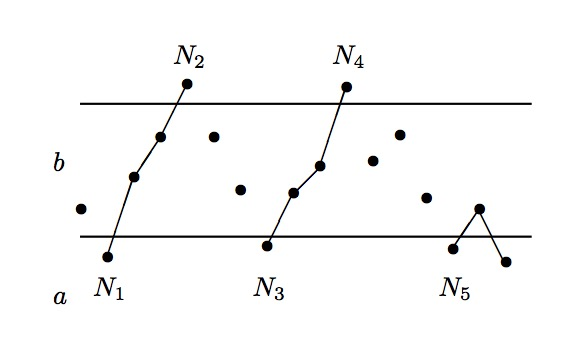
\includegraphics[width=0.6\textwidth]{week5/p_1}
\caption{Upcrossings of $[a,b]$}
\end{figure}
We may check that $\{T_k\}_{k\ge0}$ is a sequence of stopping times and is increasing:
\begin{proof}
The increasing property is trivial. To check $T_k$ is a stopping time, observe that
\begin{align*}
\{T_{2k-1}=m\} &=\left(
\bigcap_{t=T_{2k-2}+1}^{m-1} \{X_{t}<b\}
\right)\cap\{X_m\ge b\}\in\mathcal{F}_m,\\
\{T_{2k}=m\} &=\left(
\bigcap_{t=T_{2k-1}+1}^{m-1} \{X_{t}>a\}
\right)\cap\{X_m\le a\}\in\mathcal{F}_m.
\end{align*}
\end{proof}

\begin{definition}[Upcrossing]
\begin{itemize}
\item
If $T_{2k-1}<\infty$ a.s., then the sequence $X_{T_0},X_{T_1},\ldots,X_{T_{2k-1}}$ is said to \emph{upcrosses} the interval $[a,b]$ by $k$ times.
\item
Define $U_a^b[X;n]$ to be the number of upcrossing the interval $[a,b]$ by the process 
$X\triangleq \{X_k\}_{k\ge0}$ up to time $n$.
We can check that $U_a^b[X;n]$ is also a stopping time:
\[
\{U_a^b[X;n] = j\} = \{T_{2j-1}\le n<T_{2j+1}\} = \{T_{2j-1}\le n\}\cap\{T_{2j+1}\le n\}^c\in\mathcal{F}_n.
\]
We can also assert that $X_{T_{2j}}\le a$ if $T_{2j}<\infty$ a.s.; and 
$X_{T_{2j+1}}\ge b$ if $T_{2j+1}<\infty$ a.s.
\end{itemize}
\end{definition}

\begin{theorem}[Doob's Upcrossing Theorem]\label{The:upcrossing}
\begin{enumerate}
\item
Suppose that $\{X_n\}_{n\ge0}$ is a super-martingale, then for any $n\ge1, k\ge0$,
\[
\mathbb{P}\left(
U_a^b[X;n]\ge k+1
\right)\le \frac{1}{b-a}\mathbb{E}\left[
(X_n -a)^-1\{U_a^b[X;n]=k\}
\right].
\]
As a result, $\mathbb{E}[U_a^b[X;n]]\le\frac{1}{b-a}\mathbb{E}[(X_n-a)^-]$.
\item
Suppose that $\{X_n\}_{n\ge0}$ is a sub-martingale, then for any $n\ge1, k\ge0$,
\[
\mathbb{P}\left(
U_a^b[X;n]\ge k
\right)\le \frac{1}{b-a}\mathbb{E}\left[
(X_n-a)^+1\{U_a^b[X;n]=k\}
\right].
\]
As a result, $\mathbb{E}[U_a^b[X;n]]\le\frac{1}{b-a}\mathbb{E}[(X_n-a)^+]$.
\end{enumerate}
\end{theorem}

\begin{proof}
\begin{enumerate}
\item
Considering that $\{X_n\}$ is a super-martingale and $T_{(2k+1)\land n},T_{2k\land n}$ are two bounded stopping times, by Doob's Optional Sampling Theorem~\ref{The:sampling}, 
\begin{subequations}
\begin{align}
0&\ge \mathbb{E}[X_{T_{(2k+1)\land n}} - X_{T_{2k\land n}}]\nonumber\\
&=\mathbb{E}[(X_{T_{(2k+1)\land n}} - X_{T_{2k\land n}})1\{n<T_{2k}\}]
+
\mathbb{E}[(X_{T_{(2k+1)\land n}} - X_{T_{2k\land n}})1\{T_{2k}\le n<T_{2k+1}\}]
\nonumber\\&+
\mathbb{E}[(X_{T_{(2k+1)\land n}} - X_{T_{2k\land n}})1\{n\ge T_{2k+1}\}]\nonumber\\
&=\mathbb{E}[(X_{n} - X_{T_{2k}})1\{T_{2k}\le n<T_{2k+1}\}]
+
\mathbb{E}[(X_{T_{2k+1}} - X_{T_{2k}})1\{n\ge T_{2k+1}\}]\nonumber\\
&\ge
\mathbb{E}[(X_{n} - a)1\{T_{2k}\le n<T_{2k+1}\}] + \mathbb{E}[(b-a)1\{n\ge T_{2k+1}\}]\label{Eq:5:1:a}\\
&\ge 
-\mathbb{E}[(X_{n} - a)^-1\{T_{2k}\le n<T_{2k+1}\}] + (b-a)\mathbb{P}\{n\ge T_{2k+1}\}\nonumber\\
&\ge
-\mathbb{E}[(X_{n} - a)^-1\{T_{2k-1}\le n<T_{2k+1}\}] + (b-a)\mathbb{P}\{n\ge T_{2k+1}\}\nonumber
\end{align}
where (\ref{Eq:5:1:a}) is by the fact that $X_{T_{2k}}\le a, X_{T_{2k+1}}\ge b$, a.s.
Therefore, 
\begin{equation}\label{Eq:5:1:b}
\mathbb{P}\{n\ge T_{2k+1}\}\le
\frac{1}{b-a}\mathbb{E}[(X_{n} - a)^-1\{T_{2k-1}\le n<T_{2k+1}\}].
\end{equation}%T2k and T2k+1 is finite?
Note that $\{U_a^b[X;n] = k\} = \{T_{2k-1}\le n<T_{2k+1}\}$ and 
\[
\{U_a^b[X;n] \ge k+1\} = \cup_{j\ge k+1}\{U_a^b[X;n] = j\}\subseteq\{T_{2k+1}\le n\}. 
\]
Therefore, applying these two conditions on (\ref{Eq:5:1:b}) gives the desired inequality:
\[
\mathbb{P}\{U_a^b[X;n] \ge k+1\}\le\mathbb{P}\{n\ge T_{2k+1}\}\le
\frac{1}{b-a}\mathbb{E}[(X_{n} - a)^-1\{U_a^b[X;n] = k\}].
\]
Summing up the inequality above for $k\ge0$, we imply
\[
\sum_{k\ge0}\mathbb{P}\{U_a^b[X;n] \ge k+1\}\le \frac{1}{b-a}\mathbb{E}[(X_{n} - a)^-].
\]
The LHS is essentially $\mathbb{E}[U_a^b[X;n]]$:
\begin{align*}
\sum_{k\ge0}\mathbb{P}\{U_a^b[X;n] \ge k+1\}
&=\sum_{k\ge0}\sum_{j=k+1}^{\infty}\mathbb{P}\{U_a^b[X;n] = j\}
=
\sum_{j=1}^{\infty}\sum_{k=0}^{j-1}\mathbb{P}\{U_a^b[X;n] = j\}
\\&=\sum_{j=1}^{\infty}j\mathbb{P}\{U_a^b[X;n] = j\}=\mathbb{E}[U_a^b[X;n]].
\end{align*}
The proof is complete.
\end{subequations}
\item
We may use the similar technique to finish the proof on the second part.
Apply Doob's Optional Sampling Theorem~\ref{The:sampling} on $T_{(2k-1)\land n},T_{2k\land n}$
 gives
 \begin{align}
0&\ge \mathbb{E}[X_{T_{(2k-1)\land n}} - X_{T_{2k\land n}}]\nonumber\\
&=\mathbb{E}[(X_{T_{(2k-1)\land n}} - X_{T_{2k\land n}})1\{n<T_{2k-1}\}]
+
\mathbb{E}[(X_{T_{(2k-1)\land n}} - X_{T_{2k\land n}})1\{T_{2k-1}\le n<T_{2k}\}]
\nonumber\\&+
\mathbb{E}[(X_{T_{(2k-1)\land n}} - X_{T_{2k\land n}})1\{n\ge T_{2k}\}]\nonumber\\
&=\mathbb{E}[(X_{T_{2k-1}} - X_{n})1\{T_{2k-1}\le n<T_{2k}\}]
+
\mathbb{E}[(X_{T_{2k-1}} - X_{T_{2k}})1\{n\ge T_{2k}\}]\nonumber\\
&\ge
\mathbb{E}[(b - X_n)1\{T_{2k-1}\le n<T_{2k}\}] + \mathbb{E}[(b-a)1\{n\ge T_{2k}\}]\nonumber\\
&
=
\mathbb{E}[(a - X_n)1\{T_{2k-1}\le n<T_{2k}\}] + 
\mathbb{E}[(b-a)1\{T_{2k-1}\le n<T_{2k}\}] + 
\mathbb{E}[(b-a)1\{n\ge T_{2k}\}]\nonumber\\
 &=\mathbb{E}[(a - X_n)1\{T_{2k-1}\le n<T_{2k}\}] + \mathbb{E}[(b-a)1\{n\ge T_{2k-1}\}]\nonumber
 \\
 &\ge
 -\mathbb{E}[(X_n-a)^+1\{T_{2k-1}\le n<T_{2k}\}] + (b-a)\mathbb{P}\{n\ge T_{2k-1}\}\nonumber
% 
%-\mathbb{E}[(X_{n} - a)^-1\{T_{2k}\le n<T_{2k+1}\}] + (b-a)\mathbb{P}\{n\ge T_{2k+1}\}\nonumber\\
%&\ge
%-\mathbb{E}[(X_{n} - a)^-1\{T_{2k-1}\le n<T_{2k+1}\}] + (b-a)\mathbb{P}\{n\ge T_{2k+1}\}\nonumber
\end{align}
Or equivalently, 
\[
\mathbb{P}\{n\ge T_{2k-1}\}\le \frac{1}{b-a}\mathbb{E}[(X_n-a)^+1\{T_{2k-1}\le n<T_{2k}\}]
\]
Considering that $\{U_a^b[X;n] = k\} = \{T_{2k-1}\le n<T_{2k}\}$ and $\{U_a^b[X;n] \ge k\} \subseteq \{n\ge T_{2k-1}\}$, we imply
\[
\mathbb{P}\{U_a^b[X;n] \ge k\}\le \frac{1}{b-a}\mathbb{E}[(X_n-a)^+1\{U_a^b[X;n] = k\}]
\]
Summing up for $k\ge1$ both sides, we conclude the desired result.
\end{enumerate}
\end{proof}

\begin{remark}
The upcrossing of $\{X_n\}$ on the interval is the same as teh upcrossing of $\{-X_n\}$ on $[-b,-a]$.
Using this fact, we can assert that
\begin{itemize}
\item
If $\{X_n\}$ is a super-martingale, for any $n\ge1,k\ge1$,
\[
\mathbb{P}\left(
U_a^b[X;n]\ge k
\right)\le \frac{1}{b-a}\mathbb{E}\left[
(X_n -b)^-1\{U_a^b[X;n]=k\}
\right].
\]
\item
If $\{X_n\}$ is a sub-martingale, for any $n\ge1,k\ge1$,
\[
\mathbb{P}\left(
U_a^b[X;n]\ge k+1
\right)\le \frac{1}{b-a}\mathbb{E}\left[
(X_n -b)^+1\{U_a^b[X;n]=k\}
\right].
\]
\end{itemize}
\end{remark}

From the upcrossing inequality, we can easily get the result for the convergence of a martingale.
\begin{theorem}[Martingale Convergence Theorem]
Suppose that $\{X_n\}$ is a super-martingale which is ${L}^1$-bounded, i.e., $\sup_n\mathbb{E}[|X_n|]<\infty$.
Then there exists a random variable $X_\infty$. such that $X_{\infty}\in\mathcal{L}^1$, and $X_n\to X_\infty$ a.s.

If we further assume that $\{X_n\}$ is lower bounded by zero, then $\mathbb{E}[X_\infty\mid\mathcal{F}_n]\le X_n$ a.s., for any $n$.
% lower bounded by zero?
\end{theorem}
\begin{proof}
\begin{itemize}
\item
Firstly, we study the limit of $\{U_a^b[X;n]\}_{n\ge1}$, which is guaranteed to exist since 
$U_a^b[X;n]$ is increasing in $n$.
Define $U_a^b[X]\triangleq \lim_{n\to\infty}U_a^b[X;n]$, then
\begin{subequations}
\begin{align}
\mathbb{E}[U_a^b[X]]&\le \liminf_{n\to\infty}\mathbb{E}[U_a^b[X;n]]\label{Eq:5:2:a}\\
&\le \frac{1}{b-a}\liminf_{n\to\infty}\mathbb{E}[(X_n-a)^-]\label{Eq:5:2:b}\\
&\le \frac{1}{b-a}\sup_n\mathbb{E}[(X_n-a)^-]\le \frac{1}{b-a}\left(
\sup_n\mathbb{E}[|X_n|] + |a|
\right)<\infty.\nonumber
\end{align}
where (\ref{Eq:5:2:a}) is by the Fatou's lemma and (\ref{Eq:5:2:b}) is by the Doob's upcrossing Theorem~\ref{The:upcrossing}.
As a result, $U_a^b[X]<\infty$ a.s.
\end{subequations}
\item
Note that the result in the first part holds for any rational $a,b$ with $a<b$, which means that 
$\mathbb{P}(U_a^b[x]<\infty)=1,\forall a,b\in\mathbb{Q}, a<b$.
% why consider rational number
Therefore, we can show that
\[
\mathbb{P}\left[
W
\right]=0,\quad
\text{where }
W=\bigcup_{a,b\in\mathbb{Q}, a<b}
\{\liminf X_n<a<b<\limsup X_n\}.
\]
\item
Then we construct $X_\infty$ as follows.
Because of the denseness of $\mathbb{Q}$, 
for $\omega\notin W$, $X_n(\omega)$ is convergent and define $X_\infty(\omega)=\lim_{n\to\infty}X_n(\omega)$. Otherwise, define $X_n(\omega)=0$.
Then the almost sure convergence of $X_n\to X_\infty$ is obtained.

Also, we can check that $X_\infty\in\mathcal{L}^1$:
\[
\mathbb{E}[|X_\infty|]\le \liminf_{n\to\infty}\mathbb{E}[|X_n|]\le\sup_n\mathbb{E}[|X_n|]<\infty.
\]
\item
Given that $\{X_n\}$ is lower bounded by zero, the remaining result can be shown by upper bounding the integral $\int_A\mathbb{E}[X_\infty\mid\mathcal{F}_n]$ for any $A\in\mathcal{F}_n$:
\begin{subequations}
\begin{align}
\int_A\mathbb{E}[X_\infty\mid\mathcal{F}_n]&=\int_AX_\infty\diff\mathbb{P}\nonumber\\
&\le \liminf_{m\to\infty}\int_AX_m\diff\mathbb{P}\label{Eq:5:3:a}\\
&=\liminf_{m\to\infty}\int_A\mathbb{E}[X_m\mid\mathcal{F}_n]\diff\mathbb{P}\label{Eq:5:3:b}\\
&\le \liminf_{m\to\infty}\int_AX_n\diff\mathbb{P}=\int_AX_n\diff\mathbb{P}\label{Eq:5:3:c}.
\end{align}
where (\ref{Eq:5:3:a}) is by Fatou's lemma, (\ref{Eq:5:3:b}) is by the definition of conditional expectation, and (\ref{Eq:5:3:c}) is by the definition of super-martingale.
\end{subequations}
\end{itemize}
\end{proof}

\subsection{Continuous-time Martingales}
Now we discuss the concepts of martingales, super-martingales, sub-martingales for continuous-time.

\begin{definition}[Martingale]
Let $\{X_t\}_{t\ge0}$ be an adapted process on filtered probability space $(\Omega, \mathcal{F},\{\mathcal{F}_t\}_{t\ge0},\mathbb{P})$.
A stochastic process $\{X_t\}_{t\ge0}$ is called a \emph{martingale} if
\begin{enumerate}
\item
$X_t\in\mathcal{L}^1,\forall t$;
\item
$\mathbb{E}[X_{t}\mid\mathcal{F}_s] = X_s$ a.s., for all $0\le s\le t$.
\end{enumerate}
If in the last definition, ``$=$'' is replaced by ``$\le$'' or ``$\ge$'', then $\{X_t\}_{t\ge0}$
is said to be a \emph{supermartingale} or \emph{submartingale}, respectively.
\end{definition}

\begin{definition}[Optional Time]
\begin{enumerate}
\item
A mapping $T:\Omega\to[0,\infty]$ is called an $\{\mathcal{F}_t\}$-stopping time if $\{T\le t\}\in\mathcal{F}_t$ for all $t\ge0$.
\item
A mapping $T:\Omega\to[0,\infty]$ is called an $\{\mathcal{F}_t\}$-optional time if $\{T<t\}\in\mathcal{F}_t$ for all $t>0$.
\end{enumerate}
\end{definition}
It is easy to check that a stopping time is always an optional time.
Now we discuss an example about a specific optional time.

\begin{example}\label{Exp:5:1}
Let $T$ be an optional time. For each $n\ge1$, define the step-function mapping
\[
T_n = \left\{
\begin{aligned}
\frac{k}{2^n},&\quad\text{if $(k-1)/2^n\le T<k/2^n, k=1,2,\ldots$}\\
\infty,&\quad\text{if $T=\infty$}
\end{aligned}
\right.
\]
Then $\{T_n\}_{n\ge1}$ are stopping times with $T_n\downarrow T$:
\begin{itemize}
\item
To show $T_n$ is a stopping time, study the set
\begin{align*}
\{T_n\le t\}&=\bigcup_{k\ge1}\bigg[
\{T_n\le t\}\cap\left\{
\frac{k-1}{2^n}\le T<\frac{k}{2^n}
\right\}
\bigg]\\&=\bigcup_{k=1}^{\lfloor t\cdot 2^n\rfloor}\bigg[
\{T_n\le t\}\cap\left\{
\frac{k-1}{2^n}\le T<\frac{k}{2^n}
\right\}
\bigg]=\bigcup_{k=1}^{\lfloor t\cdot 2^n\rfloor}\left\{
\frac{k-1}{2^n}\le T<\frac{k}{2^n}
\right\}.
\end{align*}
Since $T$ is an optional time,
\[
\left\{
\frac{k-1}{2^n}\le T<\frac{k}{2^n}
\right\}\in\mathcal{F}_{k/2^n}\subseteq\mathcal{F}_t,\quad\forall k\le t\cdot 2^n
\implies
\{T_n\le t\}\in\mathcal{F}_t,\forall t.
\]
\item
The result for $T_n\downarrow T$ can be found in MAT3006 knowledge:
\begin{quotation}
Daniel Wong, Jie Wang. (2019) Lecture Notes
for MAT3006: Real Analysis, Lecture 19, Proposition 10.4. Available at
the link 

https://walterbabyrudin.github.io/information/Updates/Updates.html
\end{quotation}
\end{itemize}
\end{example}

\begin{definition}\label{def:5:4}
\begin{enumerate}
\item
Let $\{\mathcal{F}_t\}_{t\ge0}$ be a filteration.
Define $\mathcal{F}_{t+}\triangleq \bigcap_{s>t}\mathcal{F}_s$.
Then $\{\mathcal{F}_{t+}\}_{t\ge0}$ is also a filteration.
A filteration $\{\mathcal{F}_t\}_{t\ge0}$ is said to be \emph{right-continuous} if 
$\mathcal{F}_t = \mathcal{F}_{t+},\forall t$.

\begin{remark}
$\mathcal{F}_{t+}$ can be interpreted as the information available immediately after time $t$.
We can show that $\mathcal{F}_{t+}$ is a $\sigma$-algebra and $\mathcal{F}_{t+}\supseteq \mathcal{F}_t$.

When the filteration is right-continuous, a stopping time is the same as an optional time.
\end{remark}
\item
A filteration $\{\mathcal{F}_t\}_{t\ge0}$ is said to be \emph{complete} if each $\mathcal{F}_t$ contains all $\mathbb{P}$-null sets in $\mathcal{F}$.
\item
A filteration $\{\mathcal{F}_t\}_{t\ge0}$ is called an \emph{augmented filteration}, or said to satisfy the \emph{usual conditions}, if it is complete and right-continuous.
\end{enumerate}
\end{definition}

\section{Thursday}
\subsection{Theorems for Continuous Time Martingales}

\begin{definition}[Stopping Time $\sigma$-algebra]
Let $T$ be an $\{\mathcal{F}_t\}$-stopping time.
Define
\[
\mathcal{F}_T\triangleq \{
A\in\mathcal{F}:~A\cap\{T\le t\}\in\mathcal{F}_t,\forall t\ge0
\}.
\]
Then $\mathcal{F}_T$ is the $\sigma$-algebra for $T$,
containing the information available up to time $T$.
\end{definition}

\begin{proposition}
Let $\{\mathcal{F}_t\}$ be a filtration. Define
\begin{align*}
\mathcal{F}_{T+}&\triangleq \{A\in\mathcal{F}:~A\cap\{T\le t\}\in\mathcal{F}_{t+},~\forall t\ge0\}\\
\mathcal{G}_{T}&\triangleq \{A\in\mathcal{F}:~A\cap\{T< t\}\in\mathcal{F}_{t},~\forall t>0\}
\end{align*}
We can show that $\mathcal{F}_{T+} = \mathcal{G}_T$.
\end{proposition}

\begin{theorem}\label{The:con:mart}
\begin{enumerate}
\item
Let $\{X_t\}_{t\ge0}$ be a martingale and the filteration $\{\mathcal{F}_t\}_{t\ge0}$ satisfies the usual condition.
Then there exists a version of $\{X_t\}_{t\ge0}$, which is right-continuous with left limits, denoted as $\{\tilde{X}_t\}_{t\ge0}$.
Then $\{\tilde{X}_t\}_{t\ge0}$ is a right-continuous martingales w.r.t. $\{\mathcal{F}_t\}_{t\ge0}$.
\begin{remark}
The martingales we encountered are basically right-continuous by construction.
\end{remark}
\item
(Maximal Inequality) % assumption?
Denote $X_t^* \triangleq \sup_{s\le t}|X_s|$ as the running maximal. Then for any $t>0$ and $\lambda>0$,
\[
\mathbb{P}(X_t^*\ge\lambda)\le\frac{1}{\lambda}\mathbb{E}[|X_t|].
\]
\item
(Convergence Theorem)
Let $\{X_t\}_{t\ge0}$ be a right-continuous super-martingale, which is ${L}^1$-bounded.
Then there exists a random variable $X_\infty$ such that $X_\infty\in\mathcal{L}^1$ and $X_n\to X_\infty$ a.s.
\end{enumerate}
\end{theorem}

\begin{theorem}[Doob's Optional Sampling Theorem for Continuous-time Martingales]\label{The:5:4}
Let $\{X_t\}_{t\ge0}$ be a right-continuous martingale with the last element $X_\infty$, i.e.,
$X_\infty\in\mathcal{L}^1$ and $\mathbb{E}[X_\infty\mid\mathcal{F}_t]=X_t$ a.s. for any $t\ge0$.
Let $S\le T$ be two $\{\mathcal{F}_t\}$-optional times. 
Then $\mathbb{E}[X_T\mid\mathcal{F}_{S+}] = X_S$ a.s. 
Specifically, if $S$ is a stopping time, we replace $\mathcal{F}_{S+}$ by $\mathcal{F}_S$.
In particular, $\mathbb{E}[X_T] = \mathbb{E}[X_0]$.
\end{theorem}



Let's first show a necessary and sufficient condition for the existence of $X_\infty$:
\begin{proposition}
A last element $X_\infty$ exists if and only if $\{X_t\}_{t\ge0}$ is uniformly integrable.
\end{proposition}
\begin{proof}
Assume that $\{X_t\}_{t\ge0}$ is uniformly integrable, which implies that $\{X_t\}_{t\ge0}$ is $L^1$-bounded.
By the martingale convergence theorem~\ref{The:con:mart}, there exists a random variable $X_\infty$ such that $X_t\to X_\infty$ a.s. and $X_\infty\in\mathcal{L}^1$.
In particular, $X_t\xrightarrow{P} X_\infty$. Together with the uniform integrability of $\{X_t\}_{t\ge0}$, we can assert that $X_t\to X_\infty$ in $L^1$. % why we need the L1 convergence?
% reverse proof?
Finally, we check that $\mathbb{E}[X_\infty\mid\mathcal{F}_u] = X_u$, a.s., for any $u\ge0$, i.e., for any $A\in\mathcal{F}_u$, we have
\begin{align*}
\int_AX_\infty\diff\mathbb{P}&=\lim_{t\to\infty}\int_AX_t\diff\mathbb{P}\\
&=\lim_{t\to\infty}\int_A\mathbb{E}[X_t\mid\mathcal{F}_u]\diff\mathbb{P}
=\lim_{t\to\infty}\int_AX_u\diff\mathbb{P}=\int_AX_u\diff\mathbb{P}.
\end{align*}

Now we assume that the last element exists. 
Then $\{X_t\}$ is a collection of conditional expectations of $X_\infty$.
Applying Theorem~\ref{The:UI:condition} gives the desired result.
 


\end{proof}



Now we begin to prove Theorem~\ref{The:5:4}.
\begin{proof}
\begin{itemize}
\item
Firstly, construct the approximation of $S,T$ and argue the similar optional sampling results hold:
\begin{align*}
S_n &= \left\{
\begin{aligned}
\frac{k}{2^n},&\quad\text{if $(k-1)/2^n\le S<k/2^n, k=1,2,\ldots$}\\
\infty,&\quad\text{if $S=\infty$}
\end{aligned}
\right.
\\
T_n &= \left\{
\begin{aligned}
\frac{k}{2^n},&\quad\text{if $(k-1)/2^n\le T<k/2^n, k=1,2,\ldots$}\\
\infty,&\quad\text{if $T=\infty$}
\end{aligned}
\right.
\end{align*}
By Example~\ref{Exp:5:1}, $\{S_n\},\{T_n\}$ are two sequences of stopping times with
$S_n\downarrow S, T_n\downarrow T$.
Moroever, for each $n\ge1$, $S_n\le T_n$ a.s., taking values in a countable set.
Since $\{X_t\}_{t\ge0}$ is uniformly integrable, applying the discrete-time optional sampling theorem,
\[
\mathbb{E}[X_{T_n}\mid\mathcal{F}_{S_n}] = X_{S_n},\quad\text{a.s.}
\]
Therefore, for any $A\in\mathcal{F}_{S_n}$, $\int_AX_{T_n}\diff\mathbb{P}=\int_AX_{S_n}\diff\mathbb{P}$.
\item
We claim that $\mathcal{F}_{S+}=\cap_{n\ge1}\mathcal{F}_{S_n}$.
Therefore, for any $A\in\mathcal{F}_{S+}$,
\begin{equation}\label{Eq:5:4}
\int_AX_{T_n}\diff\mathbb{P}=\int_AX_{S_n}\diff\mathbb{P}.
\end{equation}
% show the claim
Here $\{X_{S_n}\}_{n\ge1}$ is called a backward (discrete) martingale w.r.t. $\{\mathcal{F}_{S_n}\}_{n=1}^\infty$, i.e., $\mathbb{E}[X_{S_n}\mid\mathcal{F}_{S_{n+1}}] = X_{S_{n+1}}$.
Therefore, for any $A\in\mathcal{F}_{S_{n+1}}$,
\[
\int_AX_{S_n}\diff\mathbb{P} = \int_AX_{S_{n+1}}\diff\mathbb{P}.
\]
Thus $\mathbb{E}[X_{S_{n+1}}] = \mathbb{E}[X_{S_n}] = \mathbb{E}[X_0]>-\infty$ and $\lim_{n\to\infty}\mathbb{E}[X_{S_n}]>-\infty$.
\item
We also claim that $\{X_{S_n}\}_{n\ge1}$ is uniformly integrable, which implies
$\{X_{T_n}\}_{n\ge1}$ is uniformly integrable.
Since $\{X_t\}$ is right-continuous and $T_n\downarrow T, S_n\downarrow S$, the limit of $\{X_{T_n}\}$ and $\{X_{S_n}\}$ always exist:
\[
X_T\triangleq \lim_{n\to\infty}X_{T_n} \text{ a.s.},\qquad
X_S\triangleq \lim_{n\to\infty}X_{S_n} \text{ a.s.}
\]
In particular, $X_{T_n}\to X_T$ in prob. and $X_{S_n}\to X_S$ in prob.
By Theorem~\ref{The:UI:Converge}, $X_{T_n}\to X_T$ in $L^1$ and $X_{S_n}\to X_S$ in $L^1$.
\item
Then we can show that $\mathbb{E}[X_T\mid\mathcal{F}_{S+}]=X_S$ a.s. as the follwoing.
For any $A\in\mathcal{F}_{S+}$,
\begin{align*}
\int_A\mathbb{E}[X_T\mid\mathcal{F}_{S+}]\diff\mathbb{P}
&=\int_AX_T\diff\mathbb{P}\\
&=\lim_{n\to\infty}\int_AX_{T_n}\diff\mathbb{P}\\
&=\lim_{n\to\infty}\int_AX_{S_n}\diff\mathbb{P}\\
&=\int_AX_S\diff\mathbb{P}
\end{align*}
where the second and the last equality is because of the $L^1$ convergence, and the third equality is because of (\ref{Eq:5:4}).
\item
Provided that $S$ is a stopping time, $S\le S_n$ implies $\mathcal{F}_S\subseteq\mathcal{F}_{S_n}$. Therefore, for any $A\in\mathcal{F}_S$, $\int_AX_{T_n}\diff\mathbb{P}=\int_AX_{S_n}\diff\mathbb{P}$. The proof is complete.

\end{itemize}






\end{proof}









